\documentclass{beamer}

\usepackage[utf8]{inputenc}
\usecolortheme{beaver}
\usepackage{caption}
\usepackage{subcaption}
\usepackage{todonotes}
\usepackage{bm}

\def\ci{\perp\!\!\!\!\!\perp}

\begin{document}

\title{A Simple Unified Approach to Testing High-Dimensional Conditional
Independencies for Categorical and Ordinal Data}
\author {Ankur Ankan \and Johannes Textor}
\date{}
\maketitle

\begin{frame}
	\frametitle{Overview}
	\tableofcontents
\end{frame}

\section{Motivation}
\begin{frame}
	\frametitle{Motivation: Example DAG}
	\begin{figure}
		\centering
		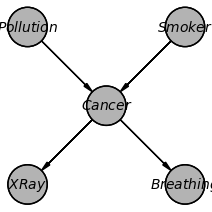
\includegraphics[scale=0.6]{imgs/example_dag.png}
		\caption*{An example Directed Acyclic Graph (DAG)}
	\end{figure}
	\begin{itemize}
		\item Directed Edges represent causal relationship between variables.
		\item DAG structures imply Conditional Independencies (CI).
		\item In the example model:
			\begin{itemize}
				\item Pollution $ \ci $ XRay $ | $ Cancer
				\item XRay $ \ci $ Breathing $ | $ Cancer
			\end{itemize}
	\end{itemize}
\end{frame}

\begin{frame}
	\frametitle{Motivation: Model Testing}
	\begin{itemize}
		\item In applied research most of these models are made by hand
			based on domain knowledge.
		\item Implied CIs can be tested in the given dataset to verify
			model structure
		\item \todo[inline]{Insert an example of model testing}
	\end{itemize}
\end{frame}

\begin{frame}
	\frametitle{Motivation: Structure Learning}
	\begin{itemize}
		\item A conditional indpendence implies that no direct causal
			link exists between the variables.
			\todo[inline]{Add a figure here}
		\item Constraint-Based algorithms like PC and FCI use these to
			learn the causal model.
	\end{itemize}
\end{frame}

\section{Background}
\begin{frame}
	\frametitle{(Conditional) Independence Test}
	\begin{block}{Independence Test}
		Two random variables $ X $ and $ Y $ are independent,
		$ X \ci Y $ if and only if $ P(X, Y) = P(X) \cdot P(Y) $.
	\end{block}

	\begin{block}{Conditional Independence Test} Two random variables $ X $
		and $ Y $ and are said to be conditionally independent given $
		\bm{Z} $, $ X \ci Y | \bm{Z} $ if and only if for all $ z $
		with $ p(z) > 0 $, $ P(X, Y | Z=z) = P(X | Z=z) \cdot P(Y |
		Z=z) $
	\end{block}
\end{frame}

\begin{frame}
	\frametitle{CI Testing is Difficult}
	\begin{itemize}
		\item Testing for conditional indpendence is a difficult problem.
		\item For continous condiitonal variables, has been proven that no single 
		      test exists which has power against all datasets.
		\item But also well studied problem, and many approaches exist.
	\end{itemize}
\end{frame}

\begin{frame}
	\frametitle{Main classes of tests}
	\begin{itemize}
		\item Stratification based tests
		\item Variable Importance based tests
		\item Residulaization based tests
	\end{itemize}
\end{frame}

\begin{frame}
	\frametitle{Stratification Based Tests}
	Most common type of test for discrete variables.
	Divides dataset into stratum based on the value of the conditional
	variables. E.g. chi-squared test.

	Problem: Looses power when number of conditonal variables are increased.
\end{frame}

\begin{frame}
	\frametitle{Variable Importance Tests}
	Compares two probablity models. E.g. SCCI

	Problems: Inherent asymmetry: The result of $ X \ci Y | Z $ can be 
	different from $ Y \ci X | Z $.
\end{frame}

\begin{frame}
	\frametitle{Residualization Based Tests}
	For linear case there are examples, none for discrete variables.
	Relies on the Daudin's theorem.

	Doesn't have the same problems as others.
\end{frame}

\section{Proposed Method}
\begin{frame}
	\frametitle{Random Forest Based Test (RFT)}
	\begin{itemize}
		\item Residualization based approach.
		\item Uses random forest as the estimator.
		\item Uses Lee-Shepherd residuals.
		\item Gives a chi-square distributed test statistic.
	\end{itemize}
\end{frame}

\begin{frame}
	\frametitle{Lee-Shepherd residuals}
	Residuals are easy for continuous case.

	Lee-Shepherd residuals for categorical and ordinal data.

	Has the important property of expection of residuals as $ 0 $ which 
	we need to use Daudin's theorem.
\end{frame}

\begin{frame}
	\frametitle{Proposition 1}
	
\end{frame}

\begin{frame}
	\frametitle{RFT: Both ordinal variables}
	$$ Q_1(\bm{x}, \bm{y}) = \frac{1}{n} \frac{(R_{\bm{x}} \cdot R_{\bm{y}})^2}{\bm{var}(R_{\bm{x}} R_{\bm{y}})} $$

	If $ X \ci Y | Z $, then asymptotically $ Q_1(\bm{x}, \bm{y}) \sim \chi^2(1) $.
\end{frame}

\begin{frame}
	\frametitle{Proposition 2}
\end{frame}

\begin{frame}
	\frametitle{RFT: One ordinal and one categorical}
	One ordinal variable and other categorical variable with $ k $ categories.
	One-hot-encoding or Dummy Variables


	$$ Q_2(\bm{x}, \bm{y}) = \frac{1}{n} (d \times \hat{\Sigma}_d^{-1} \times d^T $$

	If $ X \ci Y | Z $, then asymptotically $ Q_1(\bm{x}, \bm{y}) \sim \chi^2(k-1) $.
\end{frame}

\begin{frame}
	\frametitle{Proposition 3}
\end{frame}

\begin{frame}
	\frametitle{RFT: Both categorical}
	Both categorical variables with $ k $ and $ r $ categories.


	$$ Q_3(\bm{x}, \bm{y}) = \frac{1}{n} (d \times \hat{\Sigma}_d^{-1} \times d^T $$

	If $ X \ci Y | Z $, then asymptotically $ Q_1(\bm{x}, \bm{y}) \sim
	\chi^2((k-1)(r-1)) $.
\end{frame}

\begin{frame}
	\frametitle{Proposition 4}
\end{frame}

\begin{frame}
	\frametitle{Test summary / Algorithm}

\end{frame}

\begin{frame}
	\frametitle{Properties of RFT}
	\begin{itemize}
		\item Simple to implement
		\item Interpretable chi-square test statistic
		\item Symmetric by construction
		\item Computationally feasible
	\end{itemize}
\end{frame}

\section{Empirical Results}

\begin{frame}
	\frametitle{Empirical Analysis: Calibration}
	\begin{figure}
		\centering
		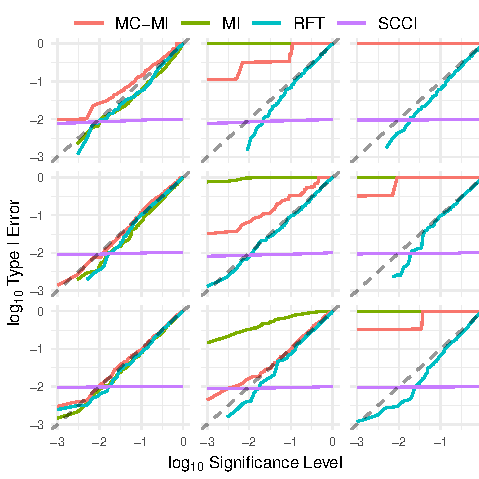
\includegraphics[scale=0.8]{imgs/calibration_add_vars.pdf}
		\caption*{Type I error vs significance level for sample sizes (top to
		bottom): $ [20, 40, 80] $ and number of conditional variables (left to
		right): $ [1, 3, 5] $ on conditionally independent simulated binary
		datasets.}
	\end{figure}
\end{frame}

\begin{frame}
	\frametitle{Empirical Analysis: Discrimination}
	\begin{figure}
		\centering
		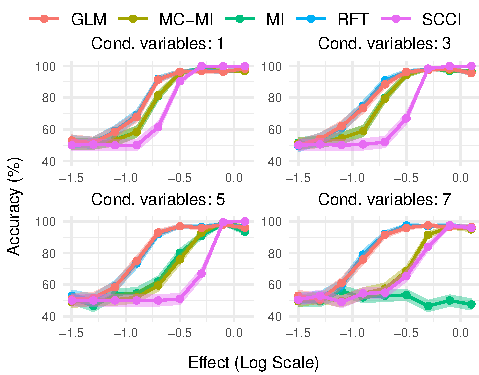
\includegraphics{imgs/accuracy.pdf}
		\caption*{Accuracy (shading: mean $\pm$ standard error, $N=200$)
		of classifying simulated binary datasets (sample size: $1000$)
		as conditionally dependent or independent.}
	\end{figure}
\end{frame}

\begin{frame}
	\frametitle{Empirical Analysis: Discrimination}
	\begin{figure}
		\centering
		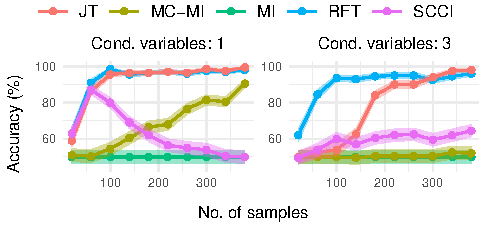
\includegraphics{imgs/accuracy_ordinal.pdf}
		\caption*{Accuracy (shading: mean $\pm$ standard error) of
		classifying simulated ordinal data (8 levels per variable) as
		conditionally dependent or independent.}	
	\end{figure}
\end{frame}

\begin{frame}
	\frametitle{Applications: Model testing}
	\begin{figure}
		\centering
		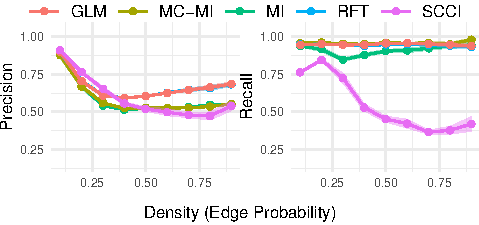
\includegraphics{imgs/model_testing.pdf}
		\caption*{Precision and recall (shading: mean $\pm$ standard
		error) of testing implied CIs and equal number of randomly
		generated CIs in binary datasets (sample size: $1000$)
		simulated from random DAGs on $ 20 $ variables.}
	\end{figure}
\end{frame}

\begin{frame}
	\frametitle{Applications: Structure Learning}
	\begin{figure}
		\centering
		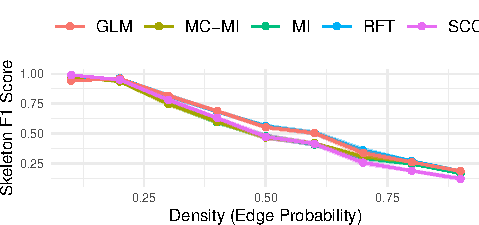
\includegraphics{imgs/sl_density.pdf}
		\caption*{Structure learning on simulated data. F1-score
		(shading: mean $\pm$ standard error) of the learned model
		skeletons for randomly generated DAGs with $20$ variables and
		varying edge probabilities.  Binary datasets of $ 1000 $
		samples are simulated from the DAGs using logistic models with
		all coefficients set to $ 0.15$.}
	\end{figure}
\end{frame}

\begin{frame}
	\frametitle{Applications: Structure Learning}
	\begin{figure}
		\centering
		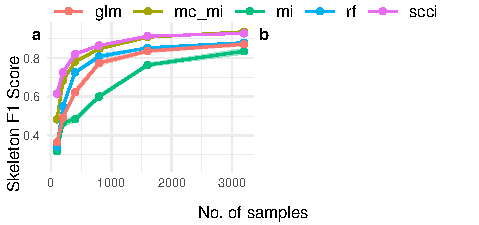
\includegraphics{imgs/sl.pdf}
		\caption*{Structure learning on (a) ``alarm'', and (b)
		``insurance'' datasets.  F1-score (shading: mean $\pm$ standard
		error, $N=10$) of the learned model skeletons.  Presence of an
		edge is considered the "positive" case for computing the
		F1-Scores.}
	\end{figure}
\end{frame}

\begin{frame}
	\frametitle{Applications: Structure Learning}
	\begin{figure}
		\centering
		\begin{subfigure}{0.5\textwidth}
			\centering
			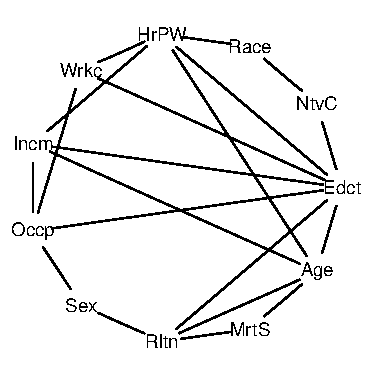
\includegraphics[scale=0.85]{imgs/sl-adult-rf.pdf}
			\caption*{}
			\label{fig:sl_adult_model}
		\end{subfigure}%
		\begin{subfigure}{0.5\textwidth}
			\centering
			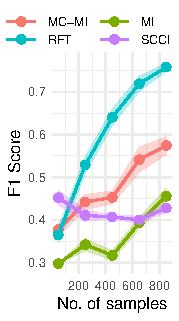
\includegraphics{imgs/adult_F1.pdf}
			\caption*{}
			\label{fig:sl_adult}
		\end{subfigure}
		\caption*{Structure learning on US census income dataset. (a)
		Learnt skeleton using RFT. (b) F1-score (shading: mean $\pm$
		standard error, $N=10$) when comparing $d$-connected variable
		pairs from the CPDAG to correlated variable pairs in the
		dataset.}
	\end{figure}
\end{frame}

\begin{frame}
	\frametitle{Runtime Analysis}
	\begin{figure}
		\centering
		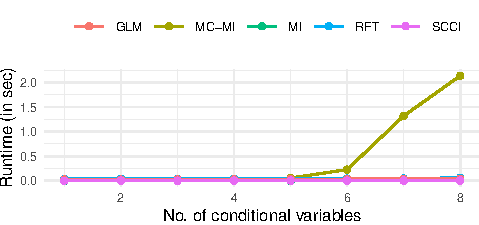
\includegraphics{imgs/runtime.pdf}
		\caption*{Runtime (shading: mean $\pm$ standard error, $N=100$)
		for CI tests with varying numbers of conditional variables and
		$1000$ samples per dataset.
		}
	\end{figure}
\end{frame}

\section{Conclusion}
\begin{frame}
	\frametitle{Conclusion}
	\begin{itemize}
		\item A simple test which works reasonably well for low
			conditional variable cases and works better than other
			for high conditional variables.
		\item Can be extended to continuous variables giving a unified
			test for working with combinations of variable types.
		\item A hybrid approach with mc-mi and rft.
	\end{itemize}
\end{frame}

% \begin{frame}
% 	Questions / Suggestions
% \end{frame}

\end{document}
